% ~~~ [ Code Coverage ] ~~~~~~~~~~~~~~~~~~~~~~~~~~~~~~~~~~~~~~~~~~~~~~~~~~~~~~~~

\subsubsection{Code Coverage}

Tracking of changes to code coverage has been tightly integrated with the CI. Travis CI has been configured to send code coverage information to the Coveralls\footnote{Coveralls - Test Coverage History \& Statistics: \url{https://coveralls.io/}} service, after each successful build. The Coveralls service tracks changes in code coverage between commits, and reports these changes when merging branches on GitHub; as illustrated in figure \ref{fig:coveralls}.

\begin{figure}[htbp]
	\begin{center}
		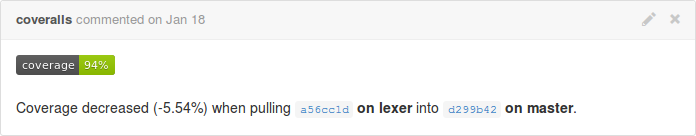
\includegraphics[width=\textwidth]{inc/8_ver/coveralls.png}
		\caption{The Coveralls service automatically reports code coverage changes when merging branches on GitHub. In this case the code coverage decreased from 100\% to 94\% when merging the LLVM IR lexer functionality.}
		\label{fig:coveralls}
	\end{center}
\end{figure}
